\documentclass{article}

\usepackage{epsfig,graphics,psfrag,color,rotating}
\usepackage{amsmath,amsfonts,amssymb,bbm}


\textwidth=30cm

\def\X{\mathcal{X}}
\def\un{\mathbbm{1}}
\def\u{\mathrm{u}}

\sloppy


\begin{document}
\thispagestyle{empty}

\begin{figure}
%
\centerline{ 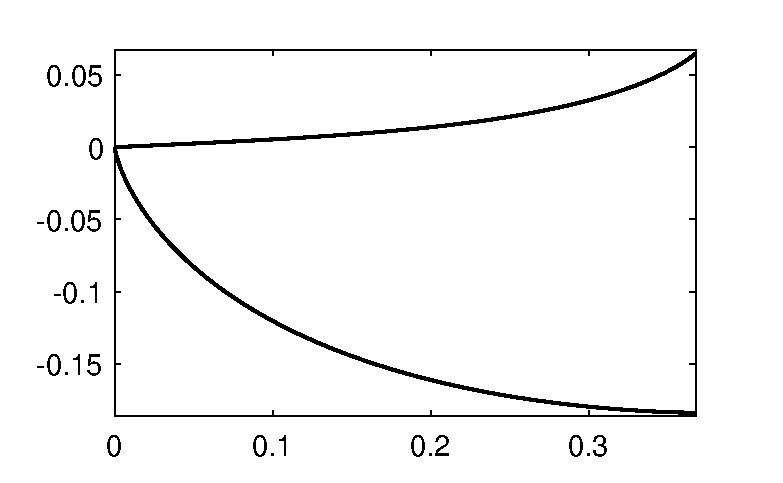
\includegraphics[width=6.5cm]{../EPS/Gamma_q2_p2} \hspace{-5mm}
  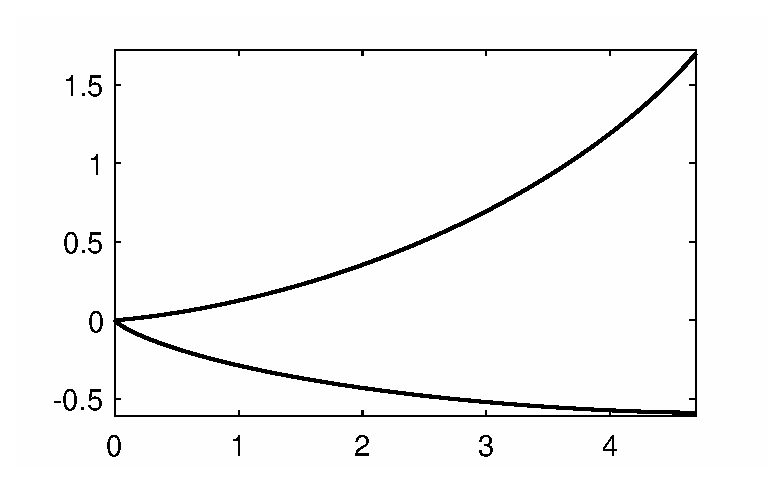
\includegraphics[width=6.5cm]{../EPS/Gamma_q5_p2}}
%
\begin{picture}(0,0)
%\put(274,28){\footnotesize $q = 2$}
\put(375,91){\footnotesize $\phi_{0,\u}$}
\put(375,33){\footnotesize $\phi_{-1,\u}$}
\put(340,6.5){\footnotesize $u$}
\put(240,62){\footnotesize \rotatebox{90}{$\phi_{k,\u}$}}
\put(277,105){\footnotesize $T_{k,1}(x) = x^2 \un_{\X_k}(x)$}
%
%\put(470,28){\footnotesize $q = 5$}
\put(558,78){\footnotesize $\phi_{0,\u}$}
\put(558,31){\footnotesize $\phi_{-1,\u}$}
\put(520,6.5){\footnotesize $u$}
\put(425,62){\footnotesize \rotatebox{90}{$\phi_{k,\u}$}}
\put(454,104){\footnotesize $T_{k,1}(x) = x^2 \un_{\X_k}(x)$}
%
\put(336,-6.25){(a)}
\put(516,-6.25){(b)}
\end{picture}
\end{figure}

\end{document}
